\documentclass[10pt,letterpaper,draftclsnofoot,onecolumn]{IEEEtran}
\usepackage[margin=0.75in]{geometry}
\usepackage{graphicx}

\begin{document}
\author{Transportation Modeling (Team 43 - Eytan Brodsky, Liang Du, Samantha Estrada, Shengjun Gu, Charles Koll)}
\title{Requirements Document: Draft 1}

\IEEEspecialpapernotice{CS 461, Fall 2018}
\maketitle

\begin{abstract}
With the inclusion of autonomous vehicles into transportation network models, the method of how they will create optimal paths is questioned as well as how they will coexist with human driven vehicles. To address this issue, we intend to investigate the pairing of connected autonomous vehicles (CAVs) with a Q-learning algorithm, aiming to gain data suggesting that vehicle autonomy and the overall infrastructure of transportation may be restructured positively to include multiple intelligent agents. Additionally, this project will explore the impact of CAVs relative to transportation congestion, using a Python based framework and vehicle models to create data on how CAVs behave on a transportation network.
\end{abstract}

\pagebreak

\section{Introduction}
	\subsection{System Purpose \& Scope}
	The purpose of this project is to provide a framework and possibly an interface to simulate the behaviors of connected autonomous vehicles in a transportation network, represented as a grid network. With this framework, models of autonomous vehicles will be created to participate in the simulation, allowing researchers to derive data on their contribution to traffic congestion.
	\subsection{System Overview}
		\subsubsection{System Context}
		This system will be used in a research environment to observe autonomous vehicles and their behavior. The data compiled from the simulations run on this system will be relevant to transportation infrastructure research and observation.
		\subsubsection{System Functions}
		Users will be able to create a city transportation system to simulate either autonomous vehicle or human vehicle status. After a simulation is run, it will provide precise data for users. By adjusting this transportation system, the data will be changed with it.
		\subsubsection{User Characteristics}
		Target users will be limited to researchers interested in transportation infrastructure, all able to navigate through the interface and understand the results of each simulation.
	\subsection{Definitions}
		\begin{itemize}
			\item CAV - Connected Autonomous Vehicle.
			\item GUI - Graphical User Interface.
			\item API - Application Programming Interface.
		\end{itemize}
\section{References}
\begin{itemize}
\item Ying Liu, Lei Liu and Wei-Peng Chen. 2017. Intelligent Traffic Light Control Using Distributed Multi-agent Q Learning. arXiv:1711.10941v1 [cs.SY]
\item Rick Zhang, Federico Rossi and Marco Pavone. 2016. Routing Autonomous Vehicles in Congested Transportation Networks: Structural Properties and Coordination Algorithms. arXiv:1603.0093v2 [cs.MA]
\item Alireza Mostafizi, Mohammad Rayeedul Kalam Siam and Haizhong Wang, Ph.D. 2018.  Autonomous Vehicle Routing Optimization in a Competitive Environment: A Reinforcement Learning Application.
\end{itemize}
\section{System Requirements}
	\subsection{Functional Requirements}
	The project should give an accurate simulation of traffic under conditions specified by the user. These conditions can include different traffic environments such as a varying number of intersections, cars, roads, etc.. The project should accurately simulate interactions between the environment and autonomous/human-controlled vehicles, taking into account factors such as acceleration, random factors for human-controlled vehicles, traffic lights, and other traffic signs.
	\subsection{Usability Requirements}
	To make this a usable interface for testing traffic routing and simulation, we will need to develop an intuitive GUI. Through this GUI, the user should be able to specify the number, position, and other parameters of variables in the environment, including cars, road layouts, traffic signals, etc.. The user should be able to simulate different conditions and have full control of the simulation.
	\subsection{Performance Requirements}
	This system is required to be able to control each vehicle in real-time. The system should collect information from each vehicle and analyze the environment to find the optimal path.
	\subsection{System Interface}
	There will be a usable API in the server-side code. It will include the vehicle destinations and location tracking. In the system interface, there will be a few optional parameters that will be changeable by the user. The user will be able to check the current status of each parameter:
	\begin{itemize}
		\item How much time will this route take
		\item How far from the start point to the destination
		\item How many intersections in the system
	\end{itemize}
	\subsection{System Modes and States}
	The program will have a start state of an empty grid representing a transportation network, with which the user will begin their interaction. From here, the user may manipulate the number or percentage of automated vehicles to the amount of human driven vehicles. They may then enter the simulation state by pressing “start” or “run”. The simulation will run for as long as the user desires, ending this state when they press “stop”.
	\subsection{Environmental Conditions}
	The program will run on Linux systems. If there is enough time we can consider writing a version that works on Windows, but Linux makes it easier to run and test on available hardware.
	\subsection{System Security}
	Security is not a major requirement for this project, since there are no network connections going outside of the local network. Without access to the physical machine, there is no risk, and even with access to the local machine there is no sensitive information in the application.
	\subsection{Information Management}
	The user should be able to record and save simulations. The user will have an option to save a simulation in some video format and a format unique to the application in order to load it into the user interface and make modifications to the simulation.
	\subsection{System Life Cycle Sustainment}
	The system will be developed until winter term, at which point it will be in its useful phase. Starting in June, unless a group decides to maintain the software, it will enter its legacy phase. It will potentially be decommissioned if another group develops a more effective product.

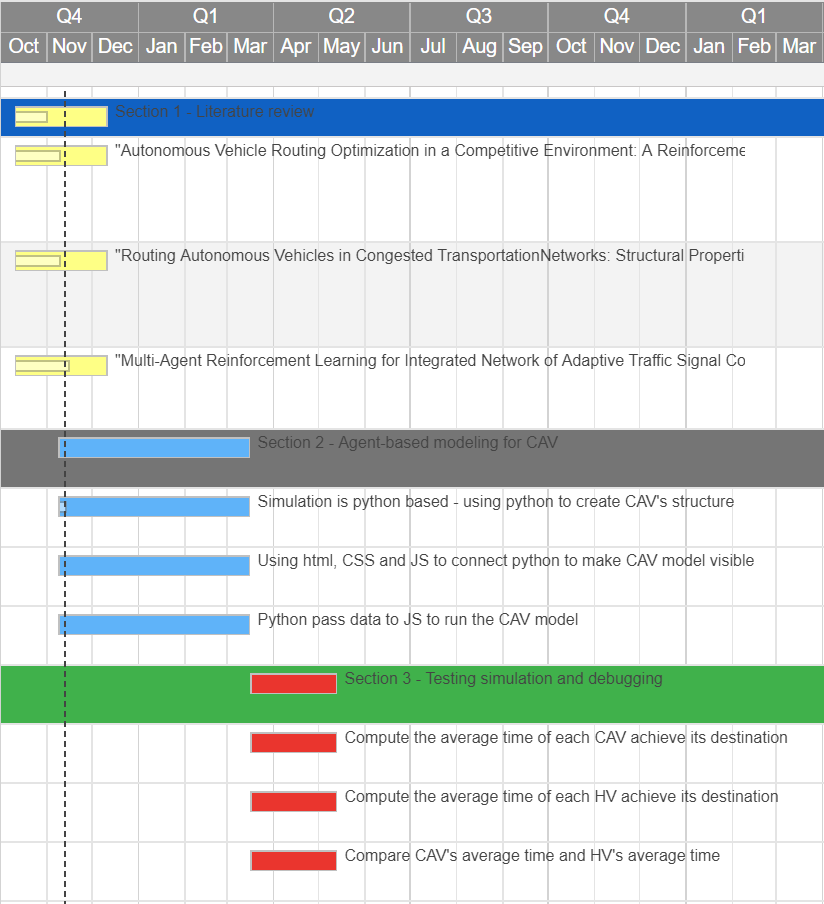
\includegraphics[width=6.5in]{gantt_chart}
\end{document}
